%package list
\documentclass{article}
\usepackage[top=3cm, bottom=3cm, outer=3cm, inner=3cm]{geometry}
\usepackage{multicol}
\usepackage{graphicx}
\usepackage{url}
%\usepackage{cite}
\usepackage{hyperref}
\usepackage{array}
%\usepackage{multicol}
\newcolumntype{x}[1]{>{\centering\arraybackslash\hspace{0pt}}p{#1}}
\usepackage{natbib}
\usepackage{pdfpages}
\usepackage{multirow}
\usepackage[normalem]{ulem}
\useunder{\uline}{\ul}{}
\usepackage{svg}
\usepackage{xcolor}
\usepackage{listings}
\lstdefinestyle{ascii-tree}{
    literate={├}{|}1 {─}{--}1 {└}{+}1 
  }
\lstset{basicstyle=\ttfamily,
  showstringspaces=false,
  commentstyle=\color{red},
  keywordstyle=\color{blue}
}
%\usepackage{booktabs}
\usepackage{caption}
\usepackage{subcaption}
\usepackage{float}
\usepackage{array}

\newcolumntype{M}[1]{>{\centering\arraybackslash}m{#1}}
\newcolumntype{N}{@{}m{0pt}@{}}


%%%%%%%%%%%%%%%%%%%%%%%%%%%%%%%%%%%%%%%%%%%%%%%%%%%%%%%%%%%%%%%%%%%%%%%%%%%%
%%%%%%%%%%%%%%%%%%%%%%%%%%%%%%%%%%%%%%%%%%%%%%%%%%%%%%%%%%%%%%%%%%%%%%%%%%%%
\newcommand{\itemEmail}{mvelasquea@unsa.edu.pe}
\newcommand{\itemStudent}{Mikhail Gabino Velasque Arcos}
\newcommand{\itemCourse}{Teoria FUNDAMENTOS DE LA PROGRAMACION II}
\newcommand{\itemCourseCode}{20214260}
\newcommand{\itemSemester}{II}
\newcommand{\itemUniversity}{Universidad Nacional de San Agustín de Arequipa}
\newcommand{\itemFaculty}{Facultad de Ingeniería de Producción y Servicios}
\newcommand{\itemDepartment}{Departamento Académico de Ingeniería de Sistemas e Informática}
\newcommand{\itemSchool}{Escuela Profesional de Ingeniería de Sistemas}
\newcommand{\itemAcademic}{2023 - B}
\newcommand{\itemInput}{Del  08 de enero del 2024}
\newcommand{\itemOutput}{Al 10 de enero del 2024}
\newcommand{\itemPracticeNumber}{20}
\newcommand{\itemTheme}{Resolución del laboratorio nuemro 20}
%%%%%%%%%%%%%%%%%%%%%%%%%%%%%%%%%%%%%%%%%%%%%%%%%%%%%%%%%%%%%%%%%%%%%%%%%%%%
%%%%%%%%%%%%%%%%%%%%%%%%%%%%%%%%%%%%%%%%%%%%%%%%%%%%%%%%%%%%%%%%%%%%%%%%%%%%

\usepackage[english,spanish]{babel}
\usepackage[utf8]{inputenc}
\AtBeginDocument{\selectlanguage{spanish}}
\renewcommand{\figurename}{Figura}
\renewcommand{\refname}{Referencias}
\renewcommand{\tablename}{Tabla} %esto no funciona cuando se usa babel
\AtBeginDocument{%
	\renewcommand\tablename{Tabla}
}

\usepackage{fancyhdr}
\pagestyle{fancy}
\fancyhf{}
\setlength{\headheight}{30pt}
\renewcommand{\headrulewidth}{1pt}
\renewcommand{\footrulewidth}{1pt}
\fancyhead[L]{\raisebox{-0.2\height}{
\includegraphics[width=3cm]{img/logo_episunsa.png}}}
\fancyhead[C]{\fontsize{7}{7}\selectfont	\itemUniversity \\ \itemFaculty \\ \itemDepartment \\ \itemSchool \\ \textbf{\itemCourse}}
\fancyhead[R]{\raisebox{-0.2\height}{
\includegraphics[width=1.2cm]{img/logo_abet}}}
\fancyfoot[L]{Estudiante Mikhail Gabino Velasque Arcos}
\fancyfoot[C]{\itemCourse}
\fancyfoot[R]{Página \thepage}

% para el codigo fuente
\usepackage{listings}
\usepackage{color, colortbl}
\definecolor{dkgreen}{rgb}{0,0.6,0}
\definecolor{gray}{rgb}{0.5,0.5,0.5}
\definecolor{mauve}{rgb}{0.58,0,0.82}
\definecolor{codebackground}{rgb}{0.95, 0.95, 0.92}
\definecolor{tablebackground}{rgb}{0.8, 0, 0}

\lstset{frame=tb,
	language=bash,
	aboveskip=3mm,
	belowskip=3mm,
	showstringspaces=false,
	columns=flexible,
	basicstyle={\small\ttfamily},
	numbers=none,
	numberstyle=\tiny\color{gray},
	keywordstyle=\color{blue},
	commentstyle=\color{dkgreen},
	stringstyle=\color{mauve},
	breaklines=true,
	breakatwhitespace=true,
	tabsize=3,
	backgroundcolor= \color{codebackground},
}

\begin{document}
	
	\vspace*{10px}
	
	\begin{center}	
		\fontsize{17}{17} \textbf{ Informe de Ejercicios teoria 03 }
	\end{center}
	\centerline{\textbf{\Large Tema: Clases}}
	%\vspace*{0.5cm}	

	\begin{flushright}
		\begin{tabular}{|M{2.5cm}|N|}
			\hline 
			\rowcolor{tablebackground}
			\color{white} \textbf{Nota}  \\
			\hline 
			     \\[30pt]
			\hline 			
		\end{tabular}
	\end{flushright}	

	\begin{table}[H]
		\begin{tabular}{|x{4.7cm}|x{4.8cm}|x{4.8cm}|}
			\hline 
			\rowcolor{tablebackground}
			\color{white} \textbf{Estudiante} & \color{white}\textbf{Escuela}  & \color{white}\textbf{Asignatura}   \\
			\hline 
			{\itemStudent \par \itemEmail} & \itemSchool & {\itemCourse \par Semestre: \itemSemester \par Código: \itemCourseCode}     \\
			\hline 			
		\end{tabular}
	\end{table}		
	
	\begin{table}[H]
		\begin{tabular}{|x{4.7cm}|x{4.8cm}|x{4.8cm}|}
			\hline 
			\rowcolor{tablebackground}
			\color{white}\textbf{Laboratorio} & \color{white}\textbf{Tema}  & \color{white}\textbf{Duración}   \\
			\hline 
			\itemPracticeNumber & \itemTheme & 04 horas   \\
			\hline 
		\end{tabular}
	\end{table}
	
	\begin{table}[H]
		\begin{tabular}{|x{4.7cm}|x{4.8cm}|x{4.8cm}|}
			\hline 
			\rowcolor{tablebackground}
			\color{white}\textbf{Semestre académico} & \color{white}\textbf{Fecha de inicio}  & \color{white}\textbf{Fecha de entrega}   \\
			\hline 
			\itemAcademic & \itemInput &  \itemOutput  \\
			\hline 
		\end{tabular}
	\end{table}
%%%%%%%%%%%%%%%%%%%%%%%%%%%%%%%%%%%%%%%%%%%%%%%%%%%%%%%%%%%%%%%%%%%%%%%%%%%%
%%%%%%%%%%%%%%%%%%%%%%%%%%%%%%%%%%%%%%%%%%%%%%%%%%%%%%%%%%%%%%%%%%%%%%%%%%%%
	\section{Tarea}
	\begin{itemize}		
		\item Basándose en la clase Soldado crear las clases Espadachín, Arquero, Caballero
y Lancero. Las cuatro clases heredan de la superclase Soldado pero aumentan
atributos y métodos, o sobrescriben métodos heredados. 
		\item  Crear la clase Mapa, que esté constituida por el tablero antes visto, que
posicione soldados en ciertas posiciones aleatorias (entre 1 y 10 soldados por
cada ejército, sólo 1 ejército por reino). Se deben generar ejércitos de 2 reinos.
No se admite guerra civil. El Mapa tiene como atributo el tipo de territorio que
es (bosque, campo abierto, montaña, desierto, playa). La cantidad de soldados,
así como todos sus atributos se deben generar aleatoriamente.
		\end{itemize}
	\section{Equipos, materiales y temas utilizados}
	\begin{itemize}
		\item Git , Git hub , clases, Diagramas UML ,herencia , herencia multiple
		\item VIM 9.0.
		\item OpenJDK 64-Bits 17.0.7.
		\item Git 2.39.2.
		\item Cuenta en GitHub con el correo institucional.
		\item Programación Orientada a Objetos.
	\end{itemize}
	
	\section{URL de Repositorio Github}
	\begin{itemize}
		\item URL del Repositorio GitHub para clonar o recuperar.
			\item URL :https://github.com/mvelasquea/fp2-23b.git

	\end{itemize}
	
	\section{Ejercicio 1:Creacion de la clase MAIN junto a clase soldado del cual deriban  la clase Arquero,Espadachin,Lancero,Caballero  y tambien el mapa el cual afecta ala batalla}
	
	\subsection{Creando la clase principal llamada "Videojuego" el cual llamara alas demas funciones las cuales permitira la creacion de la tabla y sus respectivos ejercitos}
		
	\begin{lstlisting}[language=bash,caption={CLASE MAIN o "ViDEOJUEGO"}][H]
	

import java.util.*;
public class Videojuego{
	/*
	Ejercicio lab 20 
	>	clase main 
	Autor :Mikhail Gabino Velasque Arcos

	tiempo:---
	*/
	public static void main(String[] args){
		Scanner sc = new Scanner(System.in);
		String end = "";
		do{
			Mapa terreno = new Mapa();
			terreno.genTablero();
			terreno.imprimirMapa();
			System.out.println("Ejercito 1");
			System.out.println("\u001B[32m" + terreno.getEjercito1() + "\u001B[0m");
			System.out.println("Ejercito 2");
			System.out.println("\u001B[31m" +terreno.getEjercito2()+ "\u001B[0m");

			System.out.println("\u001B[32m" + "Ejercito 1: \n " + terreno.getEjercito1().mayorVidaEjercito()+"\u001B[0m");

			System.out.println("\u001B[31m" + "Ejercito 2: \n" + terreno.getEjercito2().mayorVidaEjercito()+"\u001B[0m");


			System.out.println("\u001B[32m" + "Ranking de poder ejercito 1"+"\u001B[0m");
			terreno.getEjercito1().ranking();

			System.out.println("\u001B[31m" + "Ranking de poder ejercito 2"+"\u001B[0m");
			terreno.getEjercito2().ranking();
			
			ganador(terreno.getEjercito1().promedioPuntosEjercito(), terreno.getEjercito2().promedioPuntosEjercito());
			System.out.println("Desea salir?");
			end = sc.next();
		}while (!end.equals("si"));
	}
	public static void ganador(double vida1, double vida2){
		System.out.println("El promedio de vida del ejercito 1 es " + vida1);
		System.out.println("El promedio de vida del ejercito 2 es " + vida2);
		if(vida1 > vida2){
			System.out.println("El ejercito 1 gana el juego");
		}else if(vida2 > vida1){
			System.out.println("El ejercito 2 gana el juego");
		}else{
			System.out.println("Empate");
		}
	}
}
	\end{lstlisting}	
	
	
	\subsection{Creando la clase Soldado}
		
	\begin{lstlisting}[language=bash,caption={CLASE soldado}][H]
	



public abstract class Soldado{
	/*
	Ejercicio lab 20 
	>	clase Soldado 
	Autor :Mikhail Gabino Velasque Arcos
	tiempo:---
	*/
	protected String nombre;
	protected int nivelAtaque;
	protected int nivelDefensa;
	protected int vidaActual;
	private int velocidad;
	private String actitud = "defensiva";
	private boolean vive = true; 
	private int fila;
	private int columna;
	public Soldado(String n, int f, int c){
		this.nombre = n;
		this.fila = f;
		this.columna = c; 
		int numeroAleatorio = (int)(Math.random() * 5 + 1);
		nivelAtaque = numeroAleatorio;
		numeroAleatorio = (int)(Math.random() * 5 + 1);
		nivelDefensa = numeroAleatorio;
		velocidad = 0;
	}
	public Soldado(String n, int f, int c, int v, int a, int d){
		this(n,f,c);
		vidaActual = v;
		nivelAtaque = a;
		nivelDefensa = d;
	}
	public Soldado(){}

	public void atacar(){
		avanzar();
	}
	public void defender(){
		actitud = "defensiva";
	}
	public void avanzar(){
		velocidad++;
	}
	public void retroceder(){
		if(velocidad > 0){
			velocidad = 0;
			actitud = "defensiva";
		}else{
			velocidad--;
		}
	}
	public void serAtacado(int daño){
		vidaActual-=daño;
		if(vidaActual <= 0){
			morir();
		}
	}
	public void huir(){
		vel	ocidad+=2;
	}
	public void morir(){
			vive = false;
	}
	public void setVidaActual(int v){
		this.vidaActual = v;	
	}
	public int getVidaActual(){
		return vidaActual;
	}
	public void setFila(int f){
		this.fila = f;	
	}
	public int getFila(){
		return fila;
	}
	public void setColumna(int c){
		this.columna = c;	
	}
	public int getColumna(){
		return columna;
	}
	public String getNombre(){
		return nombre;
	}
	public int getNivelAtaque(){
		return nivelAtaque;
	}
	public int getNivelDefensa(){
		return nivelDefensa;
	}
	public boolean estaVivo(){
		return vive;
	}
	public void setNivelAtaque(int n){
		nivelAtaque = n;
	}
	public void setNivelDefensa(int n){
		nivelDefensa = n;
	}
	public void setNombre(String n){
		nombre = n;
	}
	public abstract String impresionTabla();
}
	\end{lstlisting}		
	
	
	
	\begin{lstlisting}[language=bash,caption={CLASE Lancero}][H]
	

public class Lancero extends Soldado{
		/*
		 * 	Ejercicio lab 20 
		 * 		>	clase derivada de Soldado (Lancero) 
		 * 			Autor :Mikhail Gabino Velasque Arcos
		 * 				tiempo:---
		 * 					*/
	    private int longitudLanza;
	        public Lancero(String nombre, int fila, int columna){
			        super(nombre, fila, columna);
				        int numeroAleatorio = (int)(Math.random() * 2 + 1);
							setVidaActual(numeroAleatorio);
							        longitudLanza = (int)(Math.random()*10 + 1);
								    }
		    public void schiltrom(){
			            setNivelDefensa(getNivelDefensa()+1);
				        }
		        public String impresionTabla(){
				        return "L"+this.getVidaActual();
					    }
			    public String toString(){
				            return "Nombre: " + nombre + "\n" +
						            "Nivel de Ataque: " + nivelAtaque + "\n" +
							            "Nivel de Defensa: " + nivelDefensa + "\n" +
								            "Vida Actual: " + vidaActual + "\n";
					        }
}
	\end{lstlisting}	
	
	
			
	\begin{lstlisting}[language=bash,caption={CLASE Caballero}][H]
	

public class Caballero extends Soldado {
	/*
	Ejercicio lab 20 
	>	clase derivada de Soldado (Caballero) 
	Autor :Mikhail Gabino Velasque Arcos
	tiempo:---
	*/
    private boolean modoLanza = true;
    private boolean modoEspada = false;
    private boolean montar = true;
    public Caballero(String nombre, int fila, int columna){
        super(nombre, fila, columna);
        int numeroAleatorio = (int)(Math.random() * 3 + 3);
		setVidaActual(numeroAleatorio);
    }
    public void desmontar(){
        if(montar){
            defender();
            modoEspada = true;
            modoLanza = false;
        }else{
            System.out.println("El caballero ya esta desmontado");
        }
    }
    public void montar(){
        if(!montar){
            montar = true;
            modoEspada = false;
            modoLanza = true;
            envestir();
        }else{
            System.out.println("El caballero ya esta desmontado");
        }
    }
    public void envestir(){
        if(montar){
            atacar();
            atacar();
        }else{
            atacar();
            atacar();
            atacar();
        }
    }
    public String impresionTabla(){
        return "C"+this.getVidaActual();
    }
    public String toString(){
        return "Nombre: " + nombre + "\n" +
        "Nivel de Ataque: " + nivelAtaque + "\n" +
        "Nivel de Defensa: " + nivelDefensa + "\n" +
        "Vida Actual: " + vidaActual + "\n";
    }
}
	\end{lstlisting}	
	
	\begin{lstlisting}[language=bash,caption={CLASE Espadachin}][H]
	

public class Espadachin extends Soldado {
	/*
	Ejercicio lab 20 
	>	clase derivada de Soldado (Espadachin) 
	Autor :Mikhail Gabino Velasque Arcos
	tiempo:---
	*/
    private int longitudEspada;
    public Espadachin(String nombre, int fila, int columna){

        super(nombre, fila, columna);

        int numeroAleatorio = (int)(Math.random() * 2 + 3);

		setVidaActual(numeroAleatorio);
        longitudEspada = (int)(Math.random()*10 + 1);
    }
    public void crearMuroEscudos(){
        defender();
    }
    public String impresionTabla(){
        return "E"+this.getVidaActual();
    }
    public String toString(){
        return "Nombre: " + nombre + "\n" +
        "Nivel de Ataque: " + nivelAtaque + "\n" +
        "Nivel de Defensa: " + nivelDefensa + "\n" +
        "Vida Actual: " + vidaActual + "\n";
    }
}
	\end{lstlisting}	
	
	\begin{lstlisting}[language=bash,caption={CLASE Arquero}][H]
	


public class Arquero extends Soldado{
	/*
	Ejercicio lab 20 
	>	clase derivada de Soldado (Arquero) 
	Autor :Mikhail Gabino Velasque Arcos
	tiempo:---
	*/
    private int numFlechas;
    public Arquero(String nombre, int fila, int columna){
        super(nombre, fila, columna);
        int numeroAleatorio = (int)(Math.random() * 3 + 1);
		setVidaActual(numeroAleatorio);
        numFlechas = (int)(Math.random()* 1000);
    }
    public void disparar(){
        numFlechas--;
        if(numFlechas == 0){
            System.out.println("No se puede atacar");
        }else{
            atacar();
        }
        
    }
    public String impresionTabla(){
        return "A"+this.getVidaActual();
    }
    public String toString(){
        return "Nombre: " + nombre + "\n" +
        "Nivel de Ataque: " + nivelAtaque + "\n" +
        "Nivel de Defensa: " + nivelDefensa + "\n" +
        "Vida Actual: " + vidaActual + "\n";
    }
}
	\end{lstlisting}	
		
		
	
	
	\subsection{Resultados}
	
	\begin{itemize}	
		\item Se muestra la tabla impresa con los soldados tanto del ejercito 1 como del ejercito 2 con sus respectivos atrivutos ( arquero , caballero,lancero,espadachin)y con su respectva posicion.
	\end{itemize}
	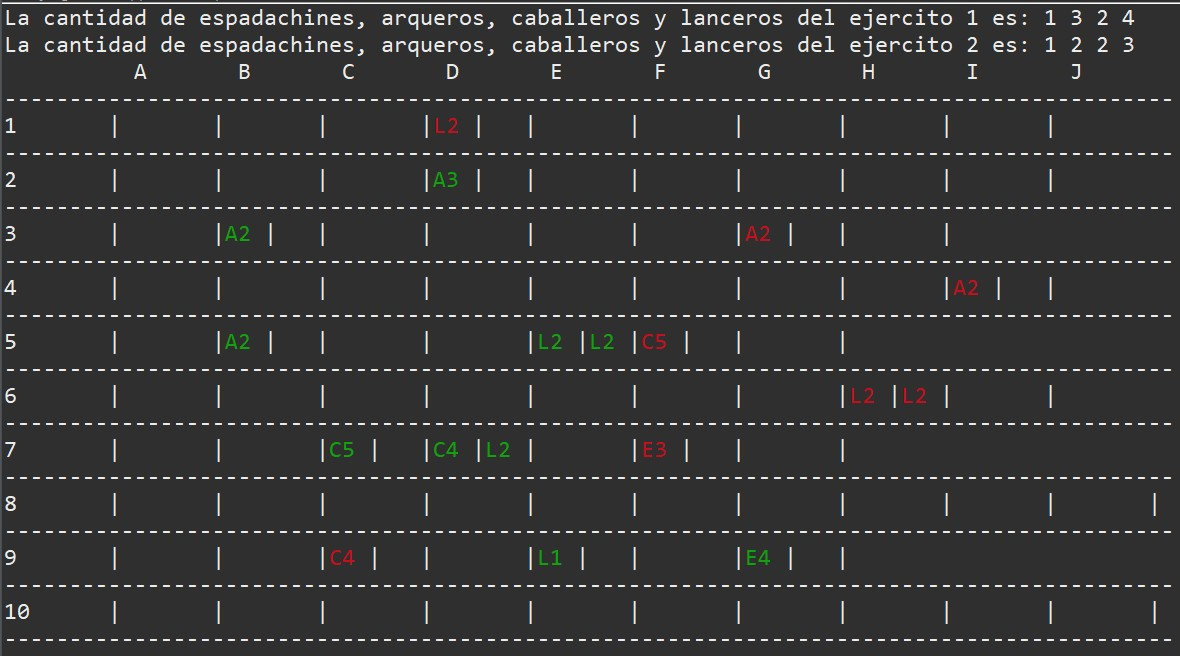
\includegraphics[scale=0.35]{img/captura1.jpeg} 	

		 
		\item Se muestra el promedio de los solados y la creacion de tales, haci como el listado,listado y caracteristicas de estos
	
	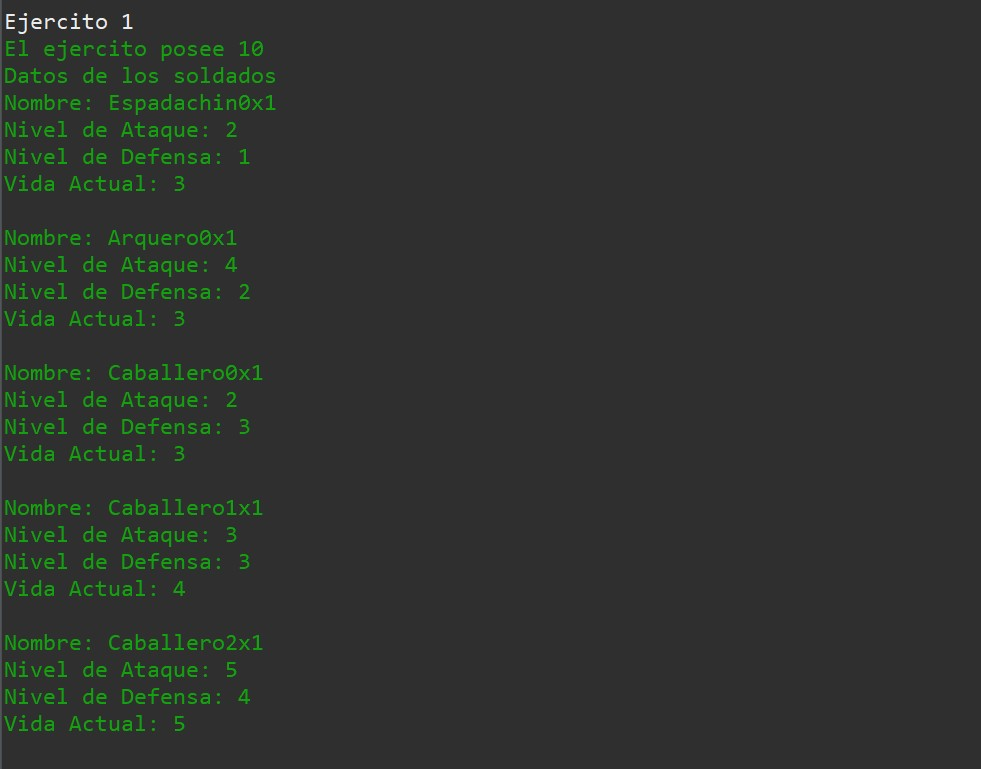
\includegraphics[scale=0.5]{img/captura2.jpeg} 
	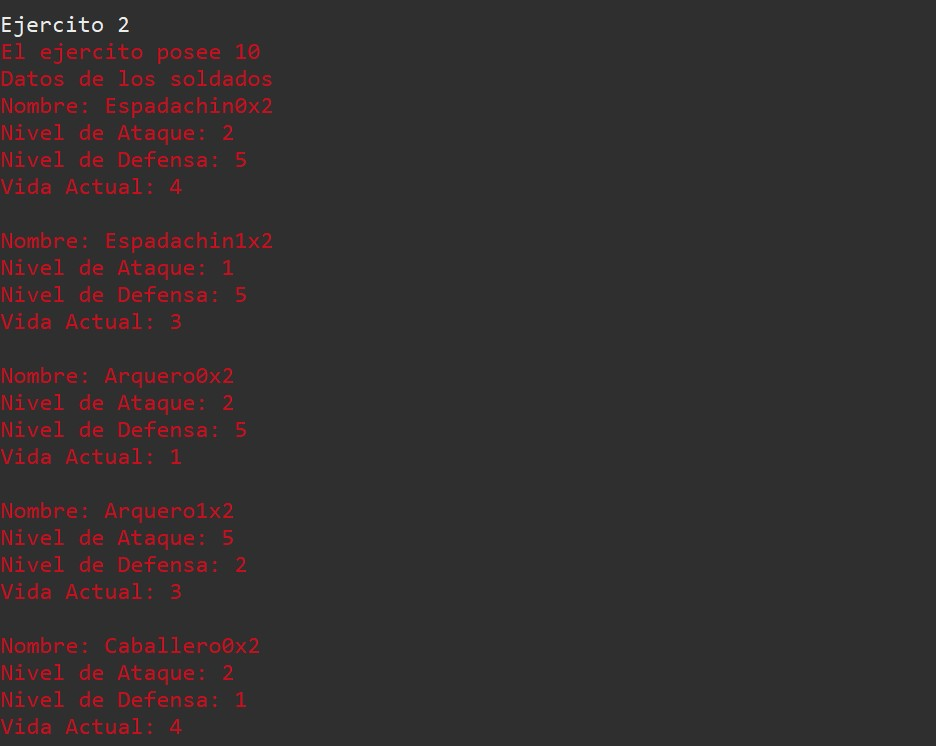
\includegraphics[scale=0.5]{img/captura3.jpeg} 
	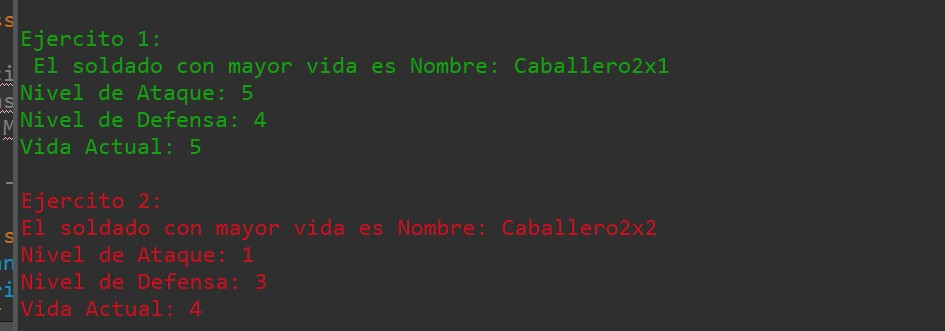
\includegraphics[scale=0.5]{img/captura4.jpeg} 
	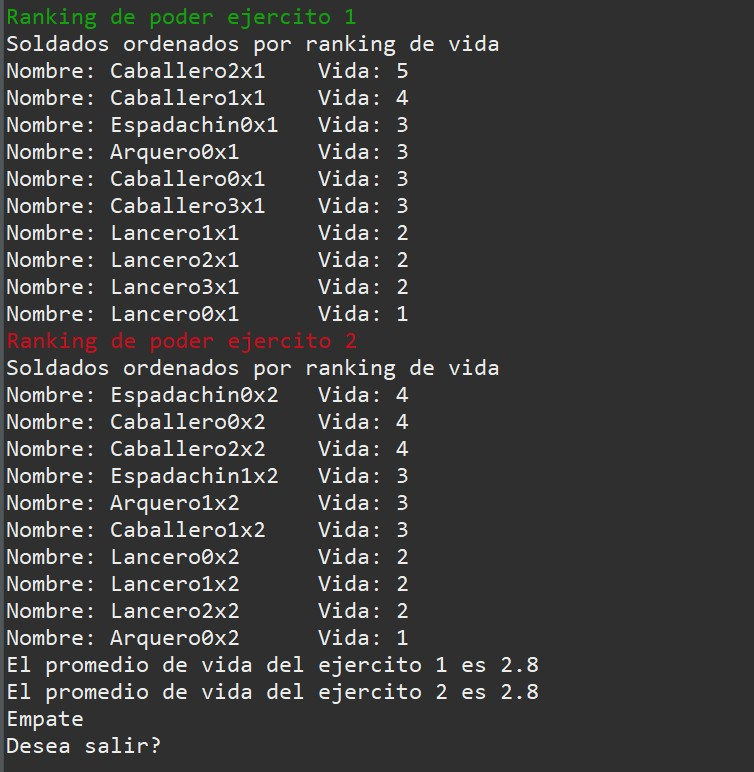
\includegraphics[scale=0.5]{img/captura5.jpeg} 
	
	
	
	\end{itemize}
	
\begin{lstlisting}[style=ascii-tree]
lab20/
|--- Videojuego.java
|--- soldado.java
|--- lancero.java
|--- gitignore.java
|--- Caballero.java
|--- Espadachin.java
|--- Arquero.java
|--- Ejercito.java
|--- Ejercito.java

|--- latex
    |--- img
    |   |--- logo_abet.png
    |   |--- logo_episunsa.png
    |   |--- logo_unsa.jpg
    |   |--- captura1.png    
    |   |--- captura2.png    

    |--- latex_Lab20_COMPLETADO.pdf    
    |--- latex_Lab20_COMPLETADO.tex
    |--- src
        |---Videojuego.java
\end{lstlisting}    













			
\end{document}